\section{Results}

\subsection{Full-Reference Fusion Metric Performance}


To interpret feature contributions, we used SHAP~\cite{shap} (SHapley Additive exPlanations) values derived from CatBoost's internal structure. SHAP values quantify how much a feature pushes the model's output away from the expected value. As shown in Fig.~\ref{fig:shap_summary}, MS-SSIM~\cite{wang2003multiscale} (Multiscale SSIM) and UQI~\cite{wang2004ssim} (Universal Quality Index) had the largest positive impact on predictions, while PSNR-B~\cite{ma2011psnr} (PSNR-Blocking), VIF\cite{sheikh2006image}, PSNR~\cite{pnsr2003} and SNR~\cite{gonzalez2002digital} (Signal-to-Noise Ratio) contributed with moderate influence. The color encoding further highlights how high and low feature values affect the model output.

\begin{figure}
    \centering
    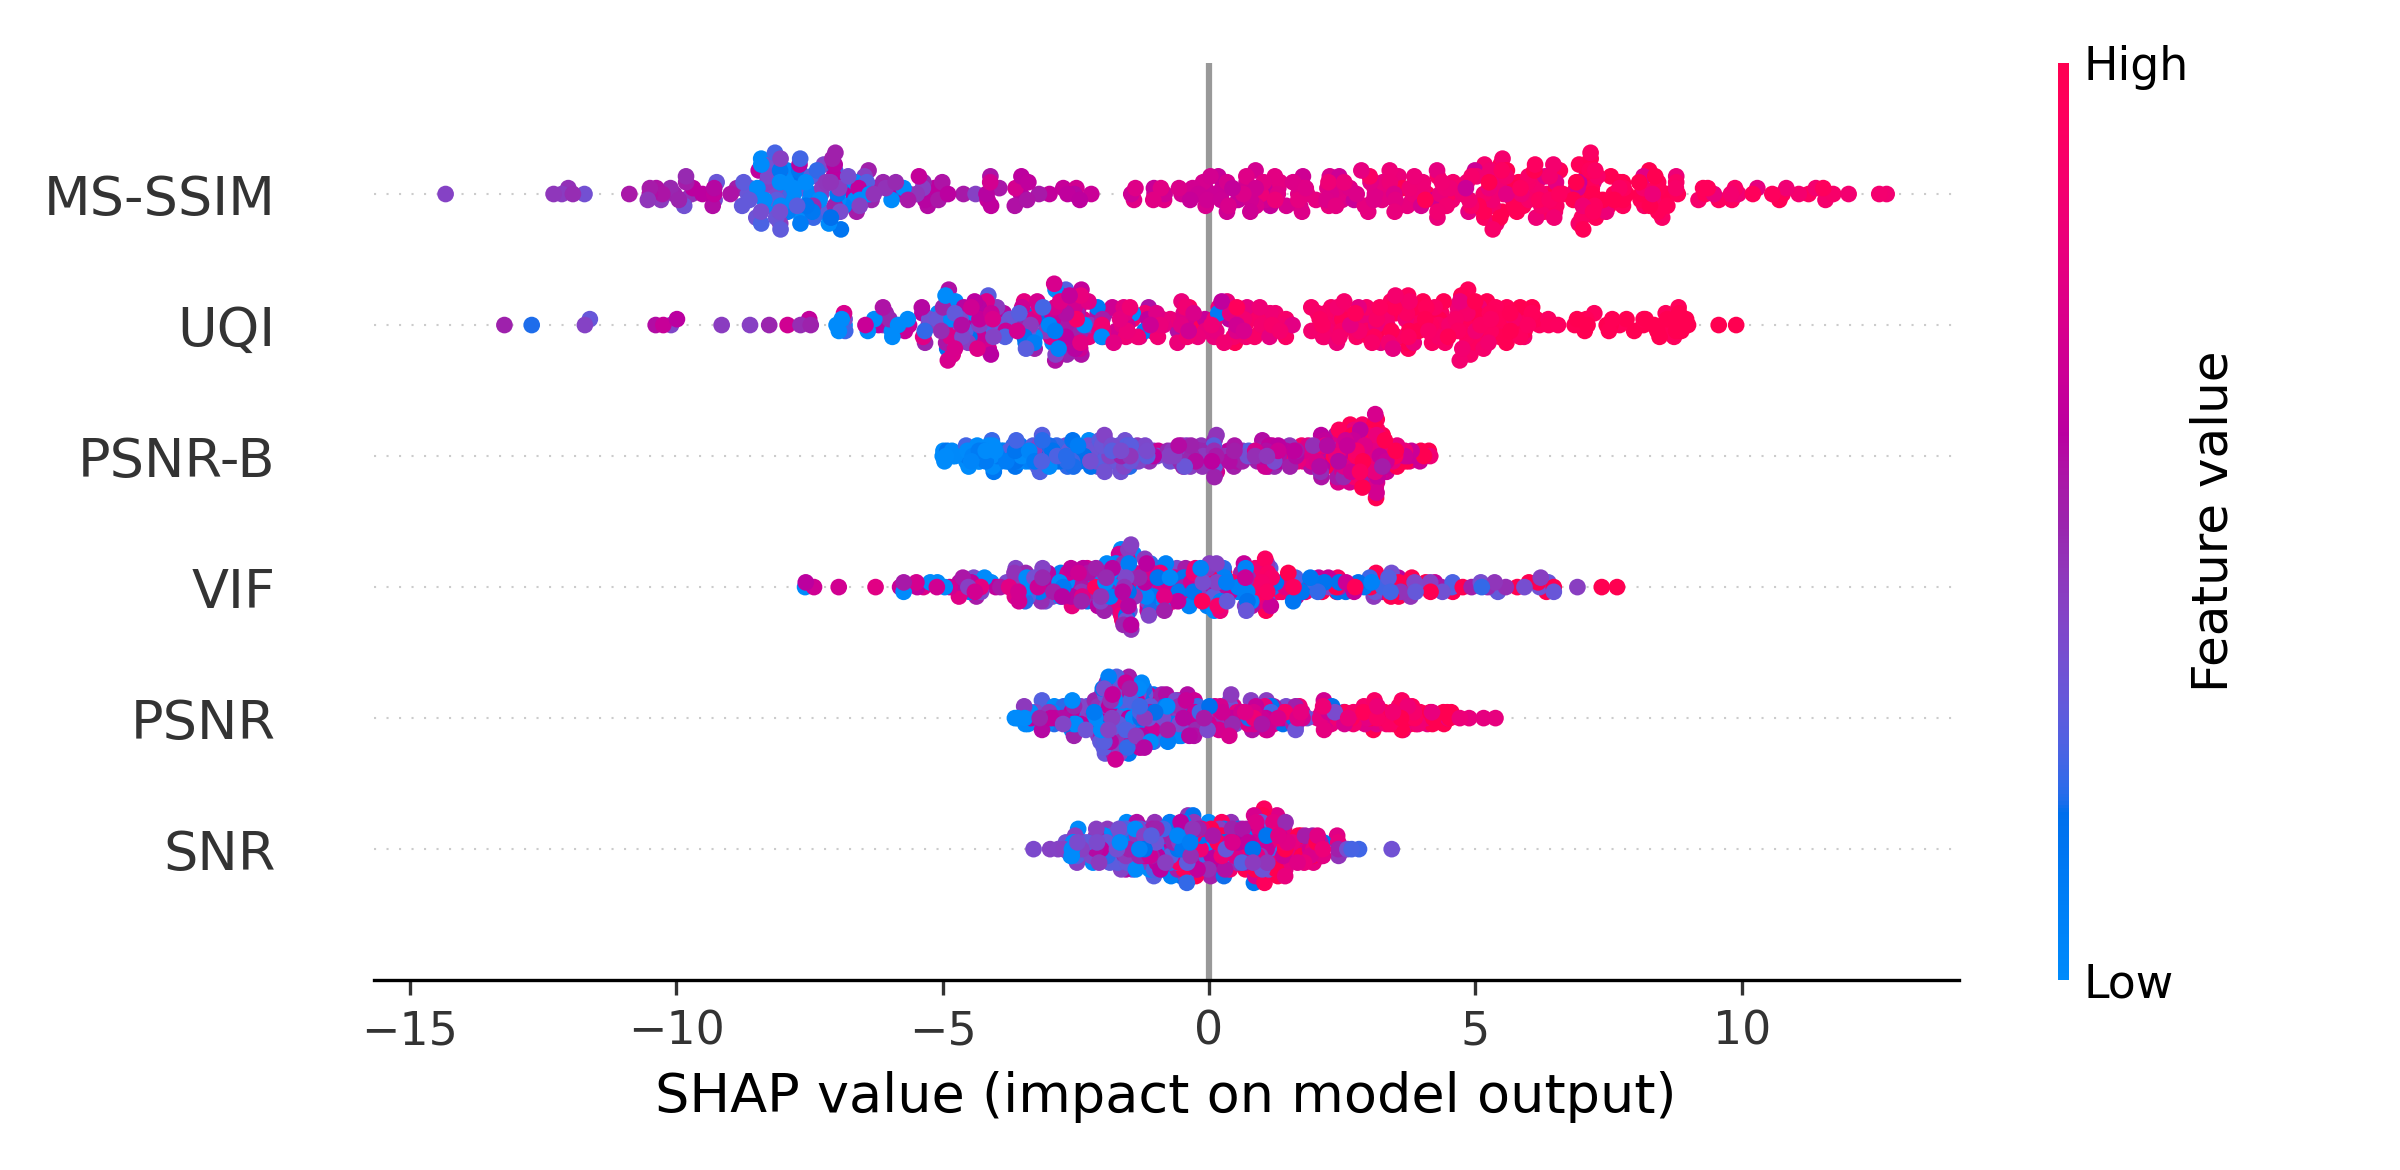
\includegraphics[width=0.7\linewidth]{images/shap_summary.png}
    \caption{SHAP summary plot for $k=6$, generated from the best CatBoost model.}\label{fig:shap_summary}
\end{figure}

When comparing the fusion metric with the individual FR metrics, Table~\ref{tab:fr_model_score} shows that the fusion metric outperformed all individual metrics in terms of PLCC, SRCC, MSE and MAE.\@ This demonstrates the effectiveness of our approach in combining multiple FR metrics to improve overall performance.

\begin{table}
\centering
\caption{Performance of our Fusion metric and the selected FR-IQA metrics. Higher PLCC and SRCC indicates better correlation with MOS.\@ Lower MSE and MAE indicate more accurate quality estimates.}\label{tab:fr_model_score}
\begin{tabular}{lcccc}
\toprule
\textbf{Metric} & \textbf{PLCC} & \textbf{SRCC} & \textbf{MSE} & \textbf{MAE} \\
\midrule
Fusion (CatBoost) & \textbf{0.8881} & \textbf{0.8893} & \textbf{65.07} & \textbf{6.160} \\
MS-SSIM & 0.7712 & 0.8489 & 2542 & 47.27 \\
PSNR & 0.8009 & 0.8132 & 420.7 & 16.57 \\
PSNR-B & 0.7996 & 0.8126 & 434.8 & 16.84 \\
SNR & 0.7931 & 0.8047 & 493.9 & 18.08 \\
VIF & 0.7723 & 0.7671 & 2584 & 47.75 \\
UQI & 0.6866 & 0.8085 & 2540 & 47.24 \\
\bottomrule
\end{tabular}
\end{table}

\subsection{No-Reference Regression Model Performance}

We refer to our NR-IQA model as pMOS-Face (pseudo-MOS for Face), reflecting its use of pseudo-MOS labels generated from the FR fusion model and its evaluation on faces. This framework can be adapted to other datasets, provided that a small set of images with human labels is available for training the FR fusion model. Fig.~\ref{fig:nr-iqa-metric} shows two evaluation scenarios: in Fig.~\ref{fig:nr-iqa-metric}(a), the model's predictions are compared against the pseudo and ground-truth MOS used during training, yielding a PLCC of 0.9285, SRCC of 0.9345, MSE of 120.2, and MAE of 9.158. Fig.~\ref{fig:nr-iqa-metric}(b) shows the predictions compared against the MOS test set, resulting in a PLCC of 0.9679, SRCC of 0.9691 and MSE of 35.34 and MAE of 4.743. These results confirm both generalization to unseen human labels and alignment with the pseudo-supervision used for training. % chktex 36

\begin{figure}[ht]
    \centering
    \begin{minipage}[t]{0.48\textwidth}
        \centering
        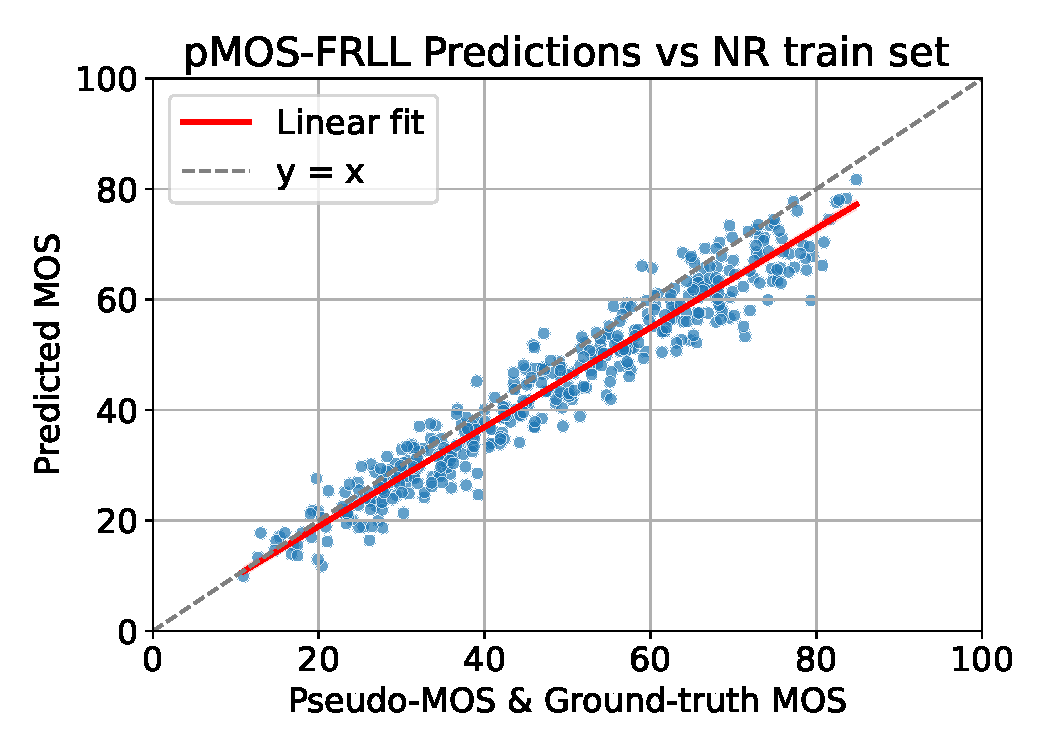
\includegraphics[width=\linewidth]{images/predictions_train.pdf}
        \textbf{(a)} Training plot.\@
    \end{minipage}
        \hfill
        \begin{minipage}[t]{0.48\textwidth}
        \centering
        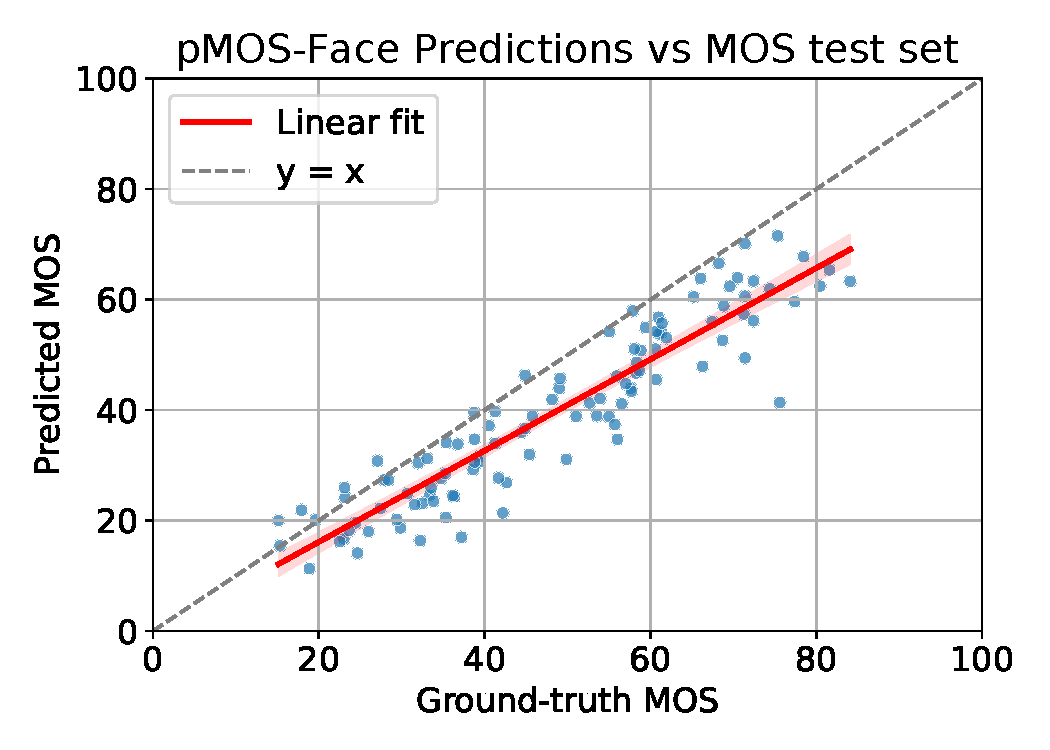
\includegraphics[width=\linewidth]{images/predictions_test.pdf}
        \textbf{(b)} Test plot.\@
    \end{minipage}
    \caption{Evaluation of our NR-IQA model. Panel (a) shows performance on the training set with pseudo and ground-truth MOS;\@ panel (b) shows performance on the disjoint test set with ground-truth MOS.}\label{fig:nr-iqa-metric}
\end{figure}

The results indicate that our model is more effective in predicting perceptual quality than classical NR-IQA metrics such as NIQE~\cite{mittal2013making} and PIQE~\cite{piqe2016}, as well as task-specific approaches like SER-FIQ~\cite{terhorst2020serfiq} and MagFace~\cite{meng2021magface}. This highlights the robustness of our weakly supervised strategy for NR-IQA on steganographically degraded facial images. Quantitative results are reported in Table~\ref{tab:nr_scores}.

\begin{table}
\centering
\caption{Performance of our pMOS-Face compared to standard NR-IQA baselines.}\label{tab:nr_scores}
\begin{tabular}{lcccc}
\toprule
\textbf{Metric} & \textbf{PLCC} & \textbf{SRCC} & \textbf{MSE} & \textbf{MAE} \\
\midrule
pMOS-Face (ours) & \textbf{0.9285} & \textbf{0.9345} & \textbf{120.6} & \textbf{9.158} \\
NIQE                 & 0.7536          & 0.7431          & 6859        & 82.62 \\
PIQE                 & 0.2993          & 0.3114          & 3297        & 57.05 \\
SER-FIQ              & -0.1648         & -0.1542         & 123.5         & 9.230 \\
MagFace              & -0.6095         & -0.6362         & 4437        & 66.24 \\
\bottomrule
\end{tabular}
\end{table}

When considering a more generalized use, where observer bias is not accounted for, our NR-IQA model shows a major improvement over the baselines. This is particularly relevant for task specific applications, where the model can be trained on a small set of images with human labels and then applied to larger datasets without the need for additional supervision. This approach allows for a more scalable and efficient solution not only for FIQA but also for other domains where reference images are not available.
